\textbf{Máster Universitario en Economía. Microeconomía Avanzada. Curso 23/24. Ejercicios 2}
\begin{center}
    \textbf{Paredes Aguilera Christian Limbert}
\end{center}
\begin{center}
	\rule{1\textwidth}{0.4pt}
\end{center}

\begin{enumerate}[\textbf{Ejercicio} 1]

    % -------------------- Ejercicio 1 --------------------
    \item \textbf{Considere una economía que consta de dos individuos que tienen unas demandas legítimas de $c_1 = 8$ y $c_2 = 12$. Calcule, para las 6 reglas presentadas en clase, las soluciones de reparto para cada una de las seis posibles dotaciones iniciales propuestas (ver tabla). Además, represente todas ellas en el gráfico adjunto.}\\

	\textbf{Solución:}
	\begin{itemize}
	    \item Regla 1: Proporcional (P). Para todo $(c,E)\in \mathcal{C}^n$,
		$$P(c,E)\equiv \lambda c,$$
	    donde $\lambda \in \mathbb{R}_+$ es tal que se alcanza el balance.
	    \item Regla 2: Ganancia igualitaria restringida (CEA). Para todo $(c,E)\in \mathcal{C}^n$,
	    $$CEA(c,E)\equiv \left(\min\left\{c_i,\lambda\right\}\right)_{i\in N}$$
	    donde $\lambda \in \mathbb{R}_+$ es tal que se alcanza el balance.
	    \item Regla 3: Pérdida igualitaria restringida (CEL). Para todo $(c,E)\in \mathcal{C}^n$,
	    $$CEL(c,E)\equiv \left(\max\left\{c_i-\lambda,0\right\}\right)_{i\in N}$$
	    donde $\lambda \in \mathbb{R}_+$ es tal que se alcanza el balance.
	    \item Regla 4: Igualitaria Restringida (CE). Para todo $(c,E)\in \mathcal{C}^n$, y cada $i\in N$,
	    $$
	    CE_i(c,E)\equiv \left\{
		\begin{array}{ll}
		    \min\left\{\frac{c_i}{\lambda}\right\} & \text{si } E\leq \sum \frac{c_j}{2},\\\\
		    \max\left\{\frac{c_i}{2},\min\left\{c_i,\lambda\right\}\right\} & \text{si } no,
		\end{array}
	    \right.
	    $$
	    donde $\lambda \in \mathbb{R}_+$ es tal que se alcanza el balance.
	    \item Regla 5: Conceder y dividir (CD). Con $|N|=2,$ para todo $(c,E)\in \mathcal{C}_n$,  
		$$CD(c,E)\equiv \left(\max\left\{E-c_j,0\right\}+\dfrac{E-\max\left\{E-c_j,0\right\}-\max\left\{E-c_i,0\right\}}{2}\right)_{i\in N}$$
	    \item Regla 6: Prioridad Secuencial (SP). Para todo $(c,E)\in \mathcal{C}^n$ y cualquier orden de prioridad $\succ_N$,
		$$SP^{\succ_N}(c,E) \equiv \left(\min\left\{c_i,\max\left\{E-\sum_{j\in N:j\succ i}c_j,0\right\}\right\}\right)_{i\in N}$$
	\end{itemize}

	\begin{center}
	    \begin{tabular}{|l|c|c|c|c|c|c|}
		\hline 
		& P & CEA & CEL & CE & CD & SP$^{1\succ 2}$ \\ 
		\hline 
		E=5 & (2.5, 2.5) & (2.5, 2.5) & (8, 12) & (2.5, 2.5) & (0, 5) & (5, 0) \\
		E=8 & (4, 4) & (4, 4) & (8, 12) & (4, 4) & (0, 8) & (8, 0) \\ 
		E=10 & (5, 5) & (5, 5) & (8, 10) & (5, 5) & (2, 8) & (8, 2) \\ 
		E=11 & (5.5, 5.5) & (5.5, 5.5) & (8, 11) & (5.5, 5.5) & (3, 8) & (8, 3) \\ 
		E=15 & (7.5, 7.5) & (7.5, 7.5) & (8, 12) & (7.5, 7.5) & (7, 8) & (8, 7) \\ 
		E=18 & (9, 9) & (8, 10) & (8, 12) & (8, 10) & (8, 10) & (8, 10) \\ 
		\hline 
	    \end{tabular} 
	\end{center}

	\begin{center}
	    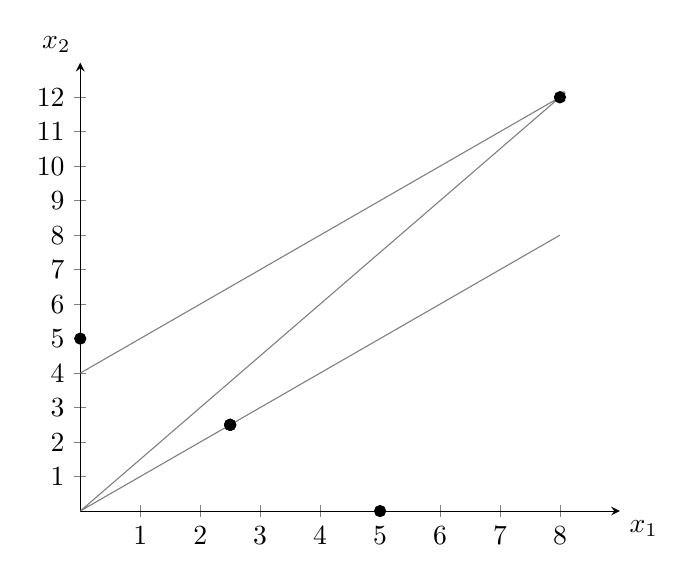
\begin{tikzpicture}
		\begin{axis}[
		    xmin=0, xmax=9,
		    ymin=0, ymax=13,
		    axis lines=center,
		    xlabel={$x_1$}, ylabel={$x_2$},
		    xtick={0,1,...,8}, ytick={0,1,...,12},
		    xlabel style={below right},
		    ylabel style={above left}
		]

		\draw[gray] (axis cs:0,4) -- (axis cs:8,12)node[]{$c$} -- (axis cs:0,0) -- (axis cs:8,8);

		% draw all coordinates of E=5
		\addplot[only marks, mark=*] coordinates {(2.5,2.5) (2.5,2.5) (8,12) (2.5,2.5) (0,5) (5,0)};
		\end{axis}
	    \end{tikzpicture}
	\end{center}

\end{enumerate}
